\documentclass[byrevtex,amssymb,aps,pra,floatfix,letterpaper]{revtex4}
\usepackage{graphicx}
\usepackage{hyperref}
\bibliographystyle{apsrev}
\date{\today}
\pagestyle{plain}
\newcommand{\degree}[0]{$^\circ$}

\begin{document}

\title{Experiment 3: Dynamic NMR spectroscopy}

\date{\today}

\maketitle

\section{Introduction}

In general spectroscopic experiments are divided into two categories: optical spectroscopy and magnetic spectroscopy. In previous experiments optical spectroscopy
based techniques (e.g., UV/VIS absorption and fluorescence) were applied to obtain information about molecules. In this experiment Nuclear Magnetic Resonance (NMR) method will be used to study molecular dynamics. NMR is the most widely applied magnetic spectroscopy method. It is an important tool for studying molecular structures and molecular dynamics of both organic and inorganic compounds. For example, for synthetic chemists it offers a great tool for identifying molecules. Another well-known magnetic resonance technique is Electron Spin Resonance (ESR; sometimes also called Electron Paramagnetic Resonance; EPR), which can be used for studying radical species.

Both NMR and ESR methods are based on the Zeeman effect, where the degenerate spin energy levels are split by an external magnetic field. In addition to the
Zeeman splitting, the possible spin -- spin interactions will modify the energetics and result in additional structure in the magnetic resonance spectra. The energy level structure of the spins is interrogated by electromagnetic radiation, which in the case of NMR is usually in the radio frequency range (MHz range) and for ESR in the microwave region (GHz range). Both optical and magnetic resonance techniques are based on interaction of the molecules with electromagnetic radiation. Both NMR and ESR are absorption experiments and thus in both experiments absorption of photons by a given sample is studied. While in the optical spectroscopy experiments the oscillating electric field component of the electromagnetic radiation induces transitions, the magnetic resonance experiment utilizes the magnetic field component of the radiation. This identifies the principal difference between the two fields of spectroscopy. A NMR spectrum displays either frequency or magnetic field (``energy'') on the $x$-axis and a quantity related to the absorption of photons on the y-axis. However, in most cases the unit for the $x$-axis is usually chosen as ppm, which represents a relative shift from a standard sample (tetramethylsilane; TMS). Note that in ESR a first derivative of the absorption is usually shown. A typical NMR spectrum is shown in Fig. \ref{fig1}. For more information on NMR and ESR spectroscopy, see Refs. \cite{ATKINS1,GUNTHER,WERTZ}.

\begin{figure}[!htp]
\begin{center}
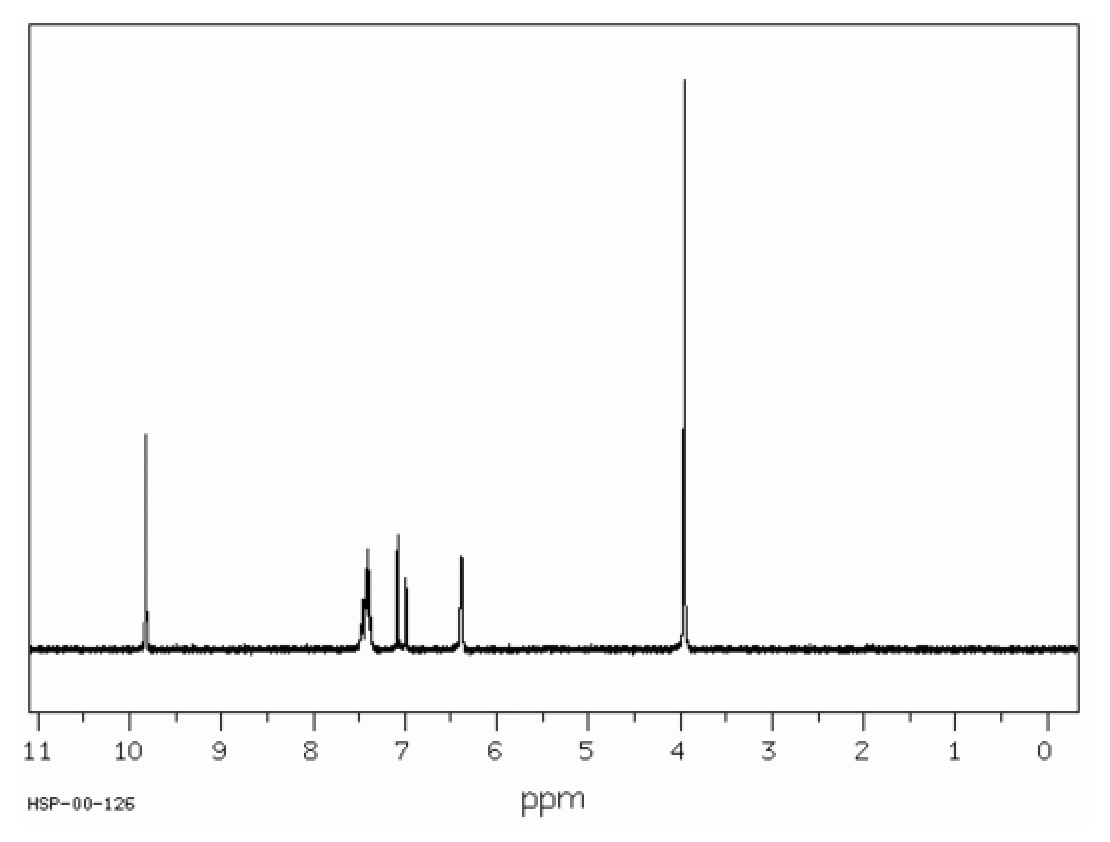
\includegraphics[scale=0.5]{fig1}
\caption{A typical proton NMR spectrum (vanillin).}
\label{fig1}
\end{center}
\end{figure}

The main objective of this experiment is to introduce the technique of dynamic NMR (DNMR) and demonstrate how it can be used to obtain information about time-
dependent molecular level phenomena. Our secondary aim is to observe the increase in the rate constant that occurs for the methyl exchange in dimethylformamide (DMF; see Fig. \ref{fig1}) as temperature is increased. The rate constants can be related to the activation energy of rotation for the C-N bond in DMF.

\begin{figure}[!htp]
\begin{center}
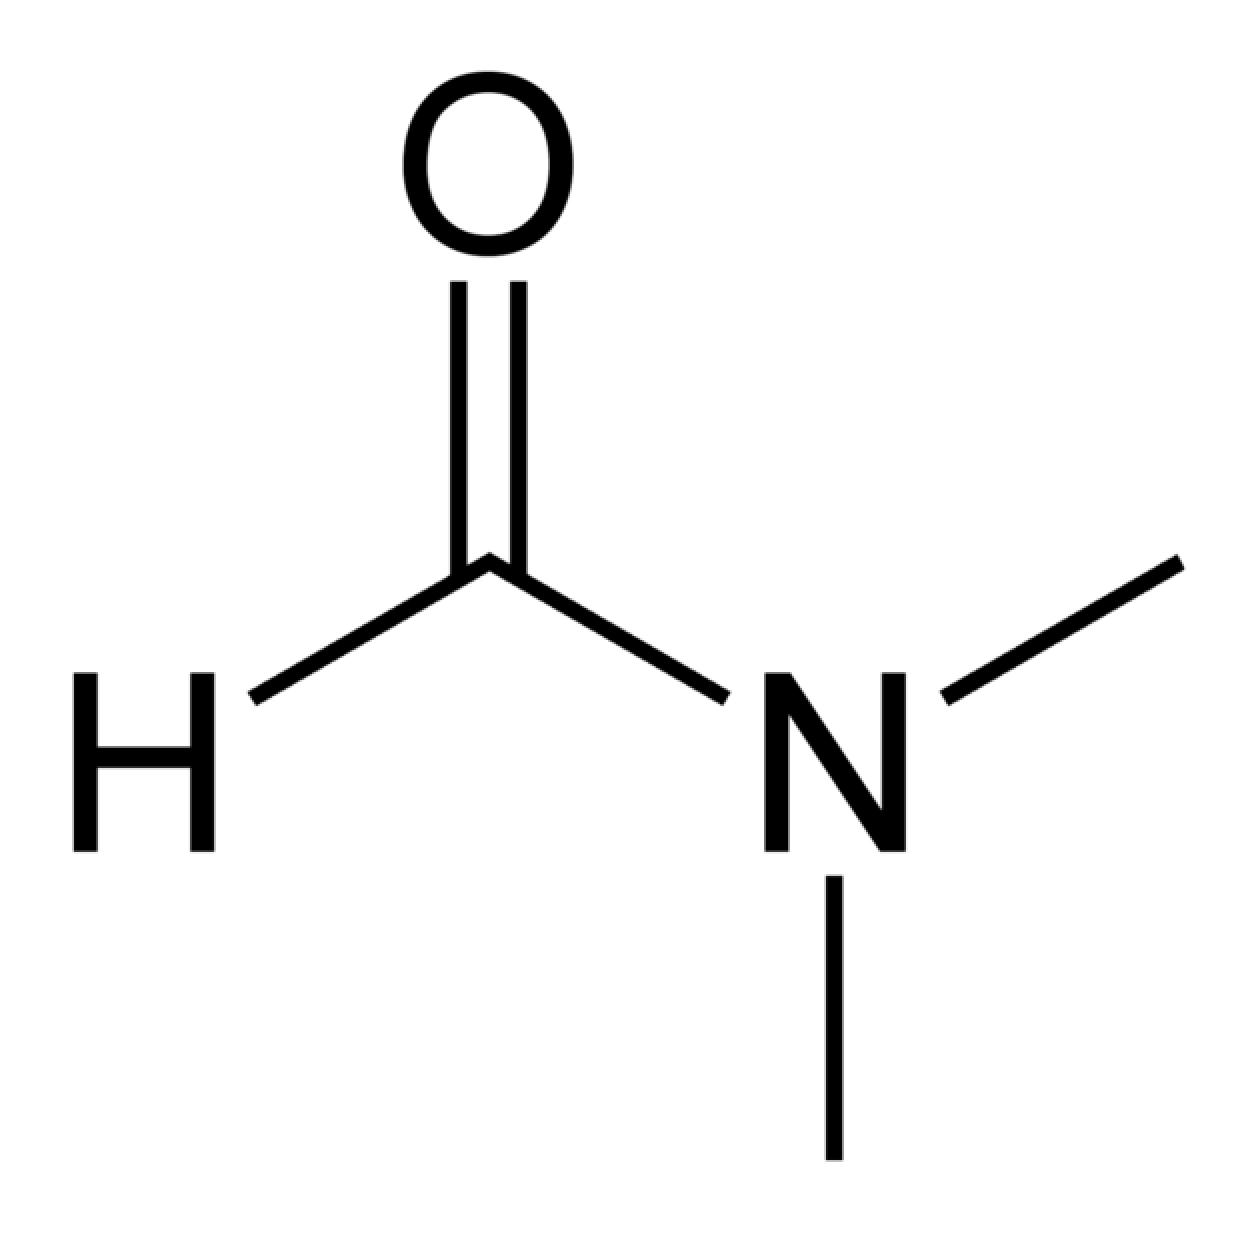
\includegraphics[scale=0.1]{fig2}
\caption{A 2-D structure of DMF.}
\label{fig2}
\end{center}
\end{figure}

\section{Theory of NMR spectroscopy}

The spin angular momentum of a proton gives rise to a magnetic moment vector $\vec{\mu}$:

\begin{equation}
\vec{\mu} = \gamma_H\vec{I}\textnormal{ with }\vec{I}=\left(\hat{I_x},\hat{I_y},\hat{I_z}\right)
\label{eq1}
\end{equation}

\noindent
where $\vec{I}$ is the nuclear spin angular momentum vector-operator with the Cartesian operator components given above and $\gamma_H$ is the magnetogyric ratio for protons ($\approx$ 2.67522 $\times$ 10$^8$ s$^{-1}$ T$^{-1}$). If an external field is placed along a given $z$-axis, we need to know the magnetic moment of the nuclear spin along that axis:

\begin{equation}
\hat{\mu_z} = \gamma_H\hat{I_z}
\label{eq2}
\end{equation}

\noindent
When this magnetic moment interacts with the external magnetic field, the Hamiltonian (i.e., the operator that yields the total energy when it operates on spin-eigenstate wavefunctions) is given by:

\begin{equation}
\hat{H} = \vec{\mu}\cdot\vec{B} \approx \hat{\mu_z} B_z = \gamma_H\hat{I_z} B_z
\label{eq3}
\end{equation}

\noindent
The spin eigenstates for a single proton are just $|+1/2>$ (or $|\alpha>$) and $|-1/2>$ (or $|\beta>$) and operating on them with the Hamiltonian of Eq. (\ref{eq3}) gives the energies of the spin levels in presence of the external magnetic field:

\begin{equation}
\hat{H}\left|\right.+\frac{1}{2}\left.\right> = \frac{1}{2}\gamma_H B_z\left|\right.+\frac{1}{2}\left.\right>\textnormal{ and }\hat{H}\left|\right.-\frac{1}{2}\left.\right> = -\frac{1}{2}\gamma_H B_z\left|\right.-\frac{1}{2}\left.\right>
\label{eq4}
\end{equation}

\noindent
Note that without the external field both spin states have the same energy (i.e., they are degenerate). In order to separate them, NMR experiment requires the external magnetic field. The energy difference between the spin levels is:

\begin{equation}
\Delta E = \gamma_H B_z
\label{eq5}
\end{equation}

\noindent
A classical analog of a proton (with nuclear spin 1/2) in a magnetic field is shown in Fig. \ref{fig3}. A classical bar magnet can have any orientation with respect to the external field but a spin can only have two orientations. The resonance condition (Eq. (\ref{eq5})) also relates the magnetic field strength units to the frequency units.

The selection rule (i.e., between which levels transitions can be observed) in NMR spectroscopy requires that there is a unit change in nuclear spin. In the above one-spin system, this corresponds to changing the nuclear spin from state $|-1/2>$ to $|+1/2>$. In ESR the requirement is that the electron spin must change by one in a transition. The selection rules become important when there are multiple spins present in the molecule and they dictate which transitions are observed experimentally.

\begin{figure}[!htp]
\begin{center}
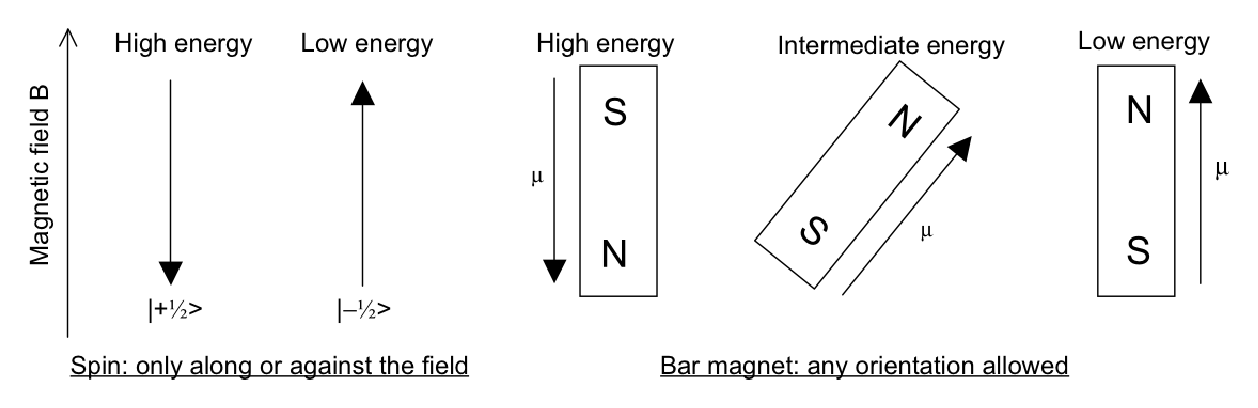
\includegraphics[scale=0.6]{fig3}
\caption{Analogy between a proton and a bar magnet in presence of external magnetic field.}
\label{fig3}
\end{center}
\end{figure}

The above one-proton example yields just one absorption line in the NMR spectrum, which is located at some fixed value of $\Delta E$. However, when a proton is
chemically bound to a molecule, the electronic structure may increase (paramagnetic contribution to shielding) or reduce (diamagnetic contribution to shielding) the local magnetic field seen by the proton. This induces a chemical shift from the free proton value. The chemical shift ($\delta$) is expressed in ppm units (see Fig. \ref{fig1}) according to the following formula:

\begin{equation}
\delta = \frac{\nu_{substance} - \nu_{TMS}}{\nu_0}
\label{eq6}
\end{equation}

\noindent
where $\nu_{vsubstance}$ is the resonance frequency for the sample (Hz), $\nu_{\textit{\tiny TMS}}$ is the resonance frequency for the TMS standard (Hz) and $\nu_0$ is the operating frequency of the spectrometer (Hz; for example, 60 MHz). The main advantage of using this scale is that it does not depend on the field strength of the NMR magnet used. Thus we conclude that each proton in a given molecule will give at least one peak in an NMR spectrum. The lines will overlap if they have identical chemical shifts or are separated from each other if they have different chemical shifts. It has been observed that based on the chemical shift, it is possible to identify where the protons are located in a molecule. Some examples are shown in Table \ref{table1}.

\begin{table}[!htp]
\caption{Chemical shifts observed for protons in different molecular environments. X denotes a halogen atom.}
\begin{tabular}{l@{\extracolsep{1cm}}l@{\extracolsep{4cm}}l@{\extracolsep{1cm}}l}
 & & & \\
Shift (ppm) & Group       &        Shift (ppm) & Group\\
-0.5 -- 0.5  & Cyclopropyl protons & 2.0 -- 4.0  & CH$_2$--N\\
0.5 -- 1.5  &  CH$_3$--C   &            2.0 -- 4.5 &  CH$_2$--X\\
0.5 -- 1.5  & CH--C        &        2.5 -- 3.5 &  CH--C$_6$H$_4$R\\
0.5 -- 4.5  & R$_2$NH      &        2.5 -- 4.5 &  CH--N\\
0.5 -- 10.0 & R--OH, alcohols  &    3.0 -- 4.0 &  CH$_3$--O\\
1.0 -- 2.0  & CH$_2$--C    &           3.0 -- 4.0 &  CH$_2$--O\\
1.0 -- 2.5  & CH$_3$--C=C  &           3.5 -- 5.5 &  CH--O\\
1.5 -- 2.5  & CH$_2$--C=C  &           4.0 -- 6.0 &  CH--X\\
1.5 -- 3.0  & CH$_3$C=O   &           4.5 -- 6.5 &  Alkenes, nonconj.\\
2.0 -- 3.0  & CH$_3$--C$_6$H$_4$R  &         5.5 -- 7.5 &  Alkenes, conjugated\\
2.0 -- 3.0  & CH$_2$--C=O  &           6.0 -- 9.0 &  Heteroaromatics\\
2.0 -- 3.0  & CH--C=O      &        6.5 -- 8.5 &  Aromatics\\
2.0 -- 3.0  & RNH$_2$      &          9.0 -- 10.5 &  H--C=O, aldehydes\\
2.0 -- 4.0  & CH$_3$--N    &           10.0 -- 13.0 & RCOOH, acids\\
\end{tabular}
\label{table1}
\end{table}

If a molecule contains multiple magnetic nuclei, or in the present case many protons, they can be magnetically coupled. You can consider a similar picture to Fig. \ref{fig3} but now you have many spins and many bar magnets. Because they are magnetic, they could interact with each other. For example, imagine turning a bar magnet when another bar magnet is close by. They feel each other and we say that they are magnetically coupled. A similar effect can be observed between two spins. In NMR this effect gives fine structure to the spectrum. Here we skip the theoretical treatment (see any of Refs. \cite{ATKINS1,GUNTHER,WERTZ} but give only a qualitative treatment. The following rules can be used to interpret a simple NMR spectrum:

\begin{enumerate}
\item If some protons have identical chemical shifts and they see the other surrounding protons the same way, we say that those protons are magnetically equivalent. They give only single resonance but show additional fine structure on the other resonances when magnetically coupled. See Fig. \ref{fig4} for an example. The distribution of lines follows the Pascal triangle as shown in Table \ref{table2}.
\item The integrated area of a proton NMR peak gives the relative number of the equivalent protons contributing to that resonance. See Fig. \ref{fig5} for an example.
\item If many magnetically non-equivalent protons couple to a given proton, complicated fine structure follows, which requires more detailed consideration.
\end{enumerate}

\begin{figure}[!htp]
\begin{center}
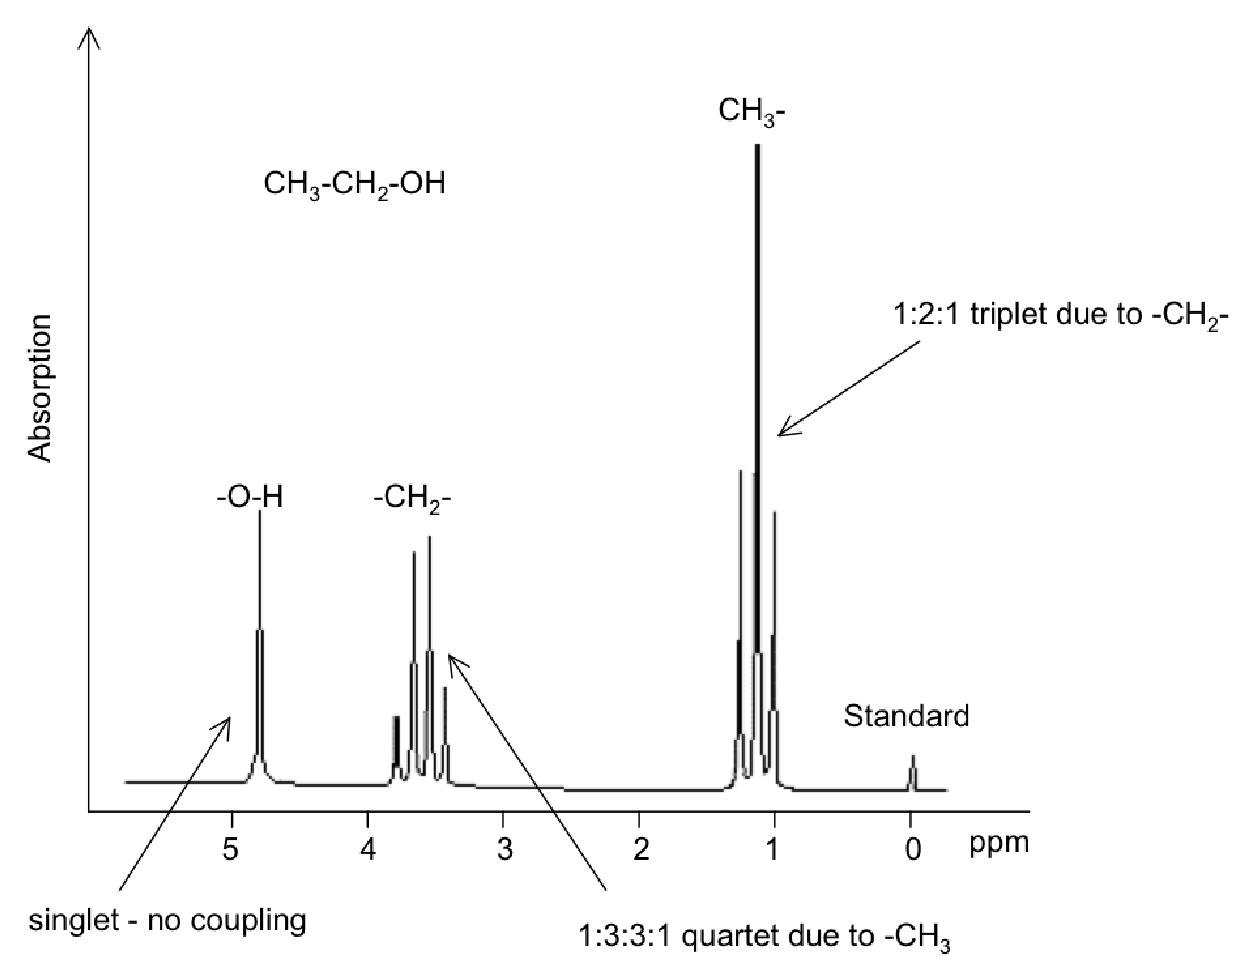
\includegraphics[scale=0.5]{fig4}
\caption{Interpretation of ethanol NMR spectrum. Note that the hydroxyl proton is not coupled to the other protons in this spectrum and it thus it gives only a singlet peak.}
\label{fig4}
\end{center}
\end{figure}

\begin{figure}[!htp]
\begin{center}
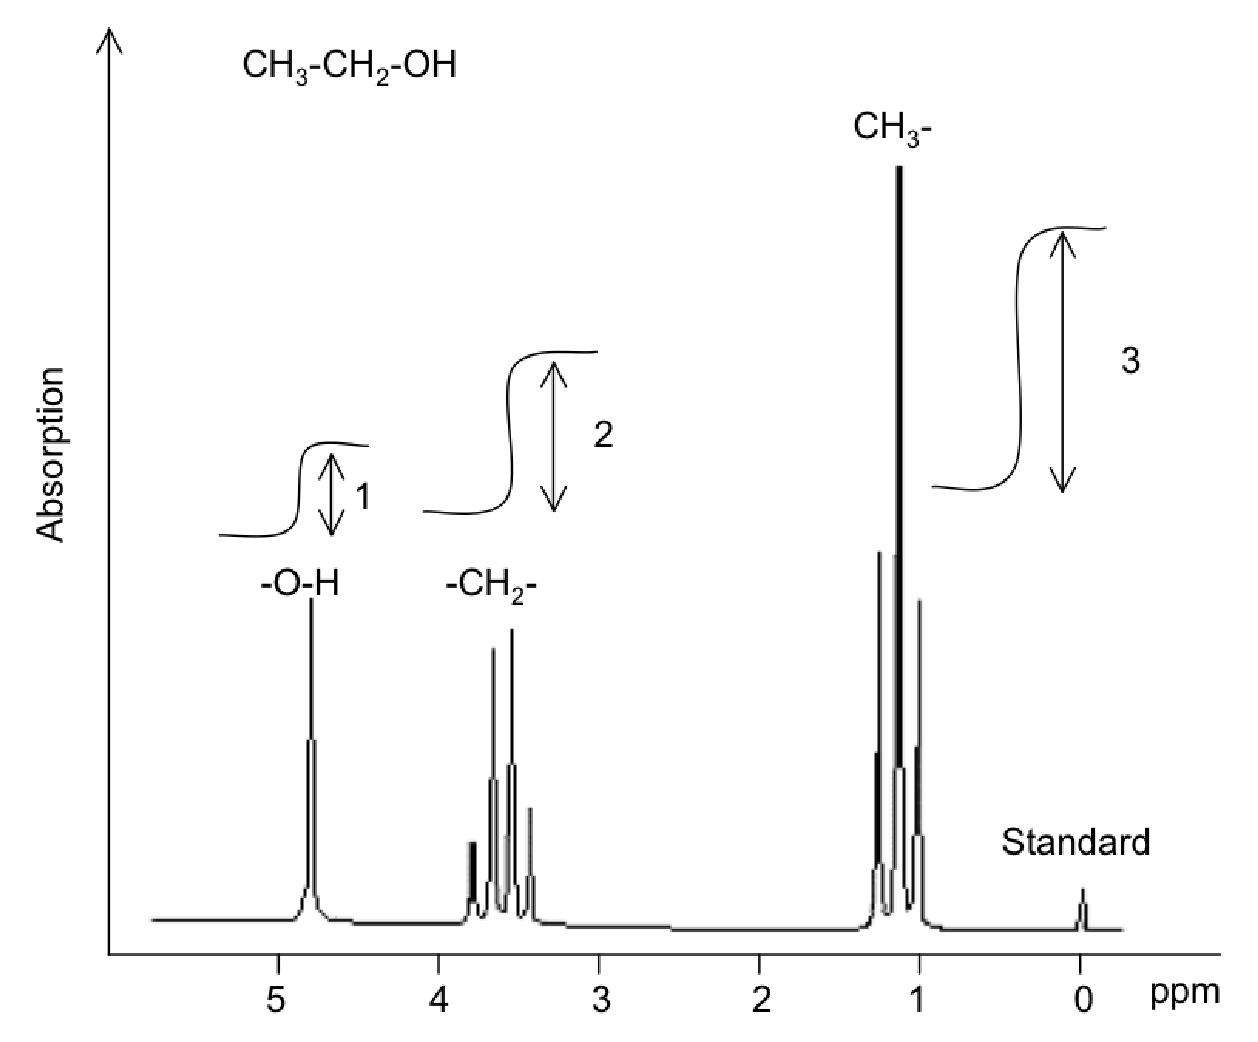
\includegraphics[scale=0.5]{fig5}
\caption{The number of equivalent protons contributing to a given resonance in NMR spectrum.}
\label{fig5}
\end{center}
\end{figure}

\begin{table}[!htp]
\caption{Pascal's triangle for interpreting proton spin-spin couplings.}
\begin{tabular}{c c c c c c c c c@{\extracolsep{3cm}}l}
 & & & 1 & & & & & & No coupling (singlet)\\
 & & 1 & & 1 & & & & & Coupling to one proton (doublet)\\
 & 1 & & 2 & & 1 & & & &  Coupling to two protons (triplet)\\
1 & & 3 & & 3 & & 1 & & & Coupling to three protons (quartet)\\
& & & ... & & & & & & \\ 
\end{tabular}
\label{table2}
\end{table}

There are two main techniques for carrying out NMR experiments: 1) scanning either the magnetic field or the frequency of the electromagnetic radiation while
monitoring the absorption of the electromagnetic field or 2) by using short pulses ($\mu$s) of electromagnetic radiation and obtaining the NMR spectrum from the free induction decay (FID) via Fourier transformation. Most modern instruments employ the pulsed technique. For more information on the techniques, see Refs. \cite{ATKINS1,GUNTHER}.

Consider the ethanol NMR spectrum in Fig. \ref{fig4} and notice that the hydroxyl proton does not seem to magnetically couple to anything. However, we would expect that it would be coupled at least to the neighboring --CH2-- but this is not seen in the spectrum. In a high-purity ethanol sample (99.99\% or so), the --OH proton shows indeed a triplet structure due to its coupling to --CH2-- protons. The main impurity in ethanol is water and therefore it appears that water has something to do with this effect. It turns out the alcohol proton undergoes rapid exchange with the solvent when water is present. If more water is gradually added to a pure ethanol sample, the NMR spectrum begins to change and finally converge to that shown in Fig. \ref{fig4}. In the intermediate water concentration regime, NMR spectroscopy can be used in estimating the alcohol proton exchange rate with water. The technique, where NMR is used in obtaining information about time-dependent phenomena, is called dynamic NMR. The main requirement for use of dynamic NMR is to have a sample where the dynamics occurs in the NMR timescale (ms range). This can be achieved, for example, by changing the water concentration in the previous ethanol example or by adjusting the sample temperature (i.e., adjusting the thermal energy available in the sample to drive dynamics). In this experiment, thermally activated internal rotational motion in DMF is studied by the dynamic NMR method. The internal mode of rotation is demonstrated in Fig. \ref{fig6}. The potential energy surface for this internal mode of rotation is periodic as shown in Fig. \ref{fig7}. Note that the potential is periodic. Do not confuse internal rotation in a molecule with molecular rotation, where the whole molecule rotates.

\begin{figure}[!htp]
\begin{center}
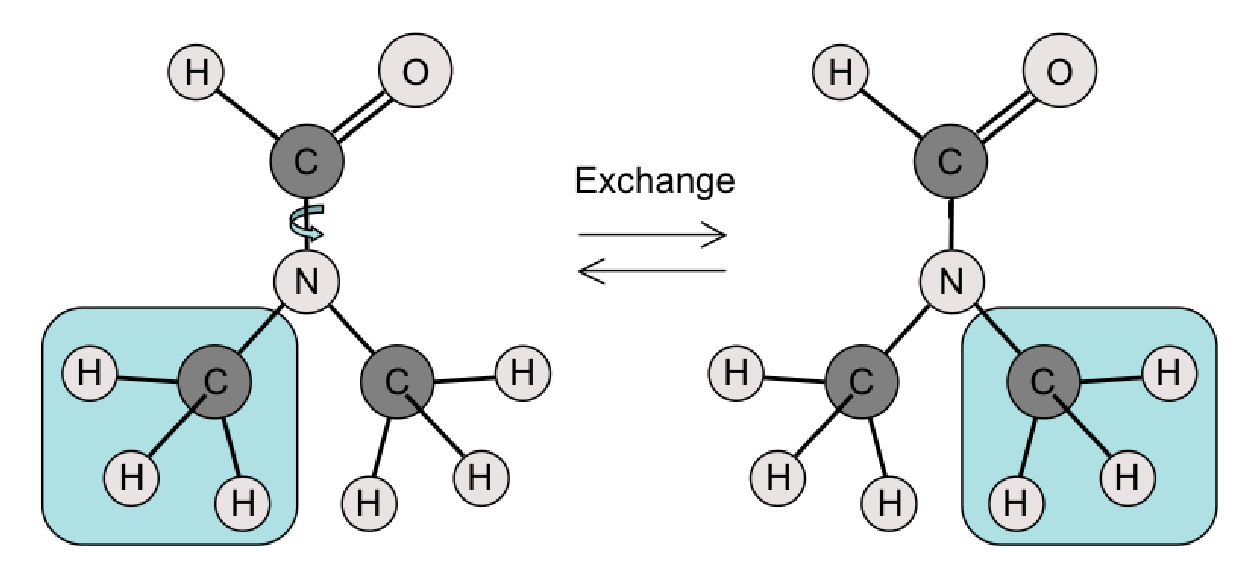
\includegraphics[scale=0.5]{fig6}
\caption{When a DMF molecule changes from one conformation (cis or trans) to another, the positions of its protons are interchanged and jump between magnetically distinct environments. Note that the energies for both conformers are equal and therefore the forward and backward reactions are equally probable.}
\label{fig6}
\end{center}
\end{figure}

\begin{figure}[!htp]
\begin{center}
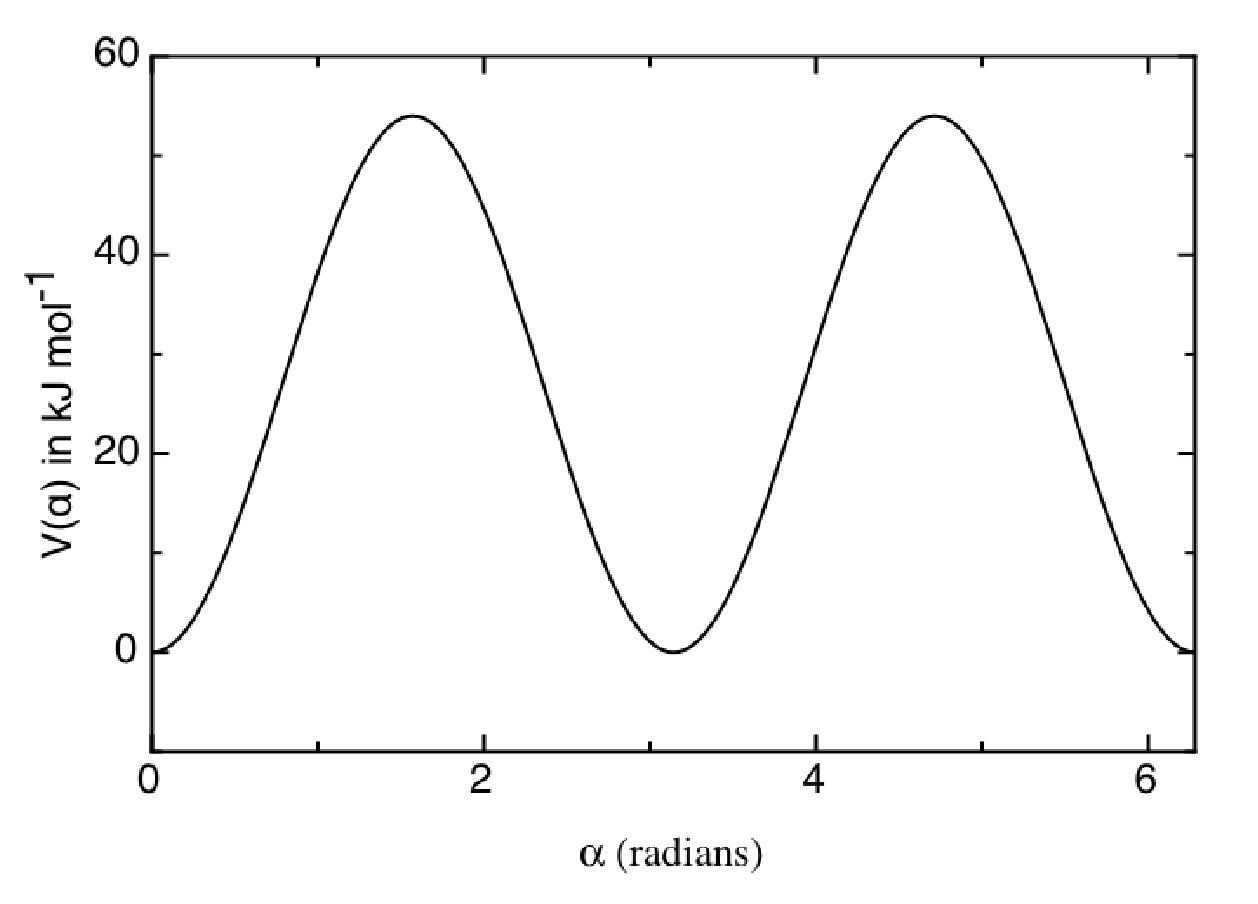
\includegraphics[scale=0.35]{fig7}
\caption{A periodic barrier to internal rotation. For example. for DMF, the minima would correspond to the two methyl-group carbons being on the same plane as C--N--O and the maxima to the case when the two carbons are both out of plane. Note that this is just an example and the magnitude of the potential does not correspond to the internal rotation in DMF.}
\label{fig7}
\end{center}
\end{figure}

When the barrier to internal rotation is only due to double bond character, as in the case of DMF, the rotation barrier can be approximated by the first term of the Fourier series:

\begin{equation}
V(\alpha) = \frac{V_0}{2}\left(1 - \cos(n\alpha)\right)
\label{eq7}
\end{equation}

\noindent
where $V_0$ is the barrier height (i.e., the energy difference between the maxima and minima) and $n$ is the number of minima on the surface. For example, in Fig. \ref{fig7} we have $V_0$ 56 kJ mol$^{-1}$ and $n = 2$. In the present case the rotating group, which consists of two methyl fragments, is sufficiently heavy that quantum mechanical treatment is not required. However, when dealing with, for example, rotation of --OH groups in hydroquinone (cis-trans isomerism), quantum mechanics cannot be ignored. In such a case, the one-dimensional Schr\"odinger equation (also called the Mathieu equation) must be solved:

\begin{equation}
-\frac{\hbar^2}{2I}\frac{\partial^2\psi_i(\alpha)}{\partial\alpha^2} + V(\alpha)\psi_i(\alpha) = E_i\psi_i(\alpha) 
\label{eq8}
\end{equation}

\noindent
where $\hbar$ is the Planck's constant (1.05457148 $\times$ 10$^{-34}$ Js), $\alpha$ is the rotation angle (rad; between 0 and 2$\pi$), $\psi_i$'s are the rotational wavefunctions, $E_i$'s are the energies of the rotational states and $I$ is the reduced moment of inertia for the rotating species (kg m$^2$). For DMF $I$ is large and hence the rotor behaves classically and zero-point energies need not to be considered (i.e., the fact that $E_0$ is larger than zero).

When the thermally induced internal rotational motion of the methyl groups (see Fig. \ref{fig6}) is slow, the NMR spectrum shows two sets of lines, one from methyl protons in each conformation (slow exchange). When the temperature is increased and the rotational motion reaches the NMR time scale, the lines begin to broaden and will finally coalesce into single broad line. When the rotational motion is fast, the spectrum shows only single narrow line at the mean of the two chemical shifts obtained in the slow motion regime (fast exchange). The maximum broadening occurs when the lifetime ($\Delta t$) of a conformation gives rise to a linewidth that is comparable to the difference in resonance frequencies ($\delta\nu$) and both broadened lines blend together into a very broad line.

Below the coalescence point (``the slow exchange limit''), the conformer lifetime can be calculated as follows. If we assume that the NMR linewidth originates solely from the rotational motion (i.e., the ``natural linewidth'' originating from the spin-lattice and spin-spin relaxation is ignored), we can obtain the conformer lifetime using the Heisenberg uncertainty principle:

\begin{equation}
\Delta E\Delta t\ge\frac{\hbar}{2}
\label{eq9}
\end{equation}

\noindent
where $\Delta E$ is the uncertainty in energy and $\Delta t$ is the conformer lifetime. The uncertainty can be obtained from the NMR linewidth (full width at half-max; FWHM) $\Delta\nu_{1/2}$ by:

\begin{equation}
\Delta E = h\Delta\nu_{1/2}
\label{eq10}
\end{equation}

\noindent
Note that here we assume that $\Delta\nu_{1/2}$ is only due to exchange (i.e., other broadening mechanisms are not active). Combining the Eqs. (\ref{eq9}) and (\ref{eq10}) gives:

\begin{equation}
\Delta t\ge\frac{1}{4\pi\Delta\nu_{1/2}}
\label{eq11}
\end{equation}

Note that because of the inequality the above calculation gives only the relative magnitude for the lifetime correctly. In order to get the magnitude correctly, one would have to use the Bloch equations for deriving $\Delta t$ \cite{GUNTHER}. This gives the following absolute magnitude for the lifetime:

\begin{equation}
\Delta t = \frac{1}{\pi\Delta\nu_{1/2}}
\label{eq12}
\end{equation}

At the point of coalescence a similar uncertainty principle derivation could be used, but it would only give the right relative magnitude. A more rigorous approach using the Bloch equations gives:

\begin{equation}
\Delta t = \frac{\sqrt{2}}{\pi\delta\nu}
\label{eq13}
\end{equation}

\noindent
where equal concentrations were assumed for both conformers. For example, if the chemical shifts of two lines differ by 100 Hz, the spectrum collapses into a single line when the conformation lifetime is about 5 ms. Note that the separation of the lines must be given in Hz and not, for example, in ppm.

In the fast exchange limit only one line appears and the following approximation (derived from the Bloch equations) holds:

\begin{equation}
\Delta t = \frac{2\Delta\nu_{1/2}}{\pi\left(\delta\nu\right)^2}
\label{eq14}
\end{equation}

\noindent
where $\delta\nu$ is the separation between the lines in the slow exchange case.

\section{Kinetics}

The conformation change in DMF is a first order kinetic process. As such the first order rate constant $k_1$ is inversely proportional to the conformer lifetime $\Delta t$:

\begin{equation}
k_1 = \frac{1}{\Delta t}
\label{eq15}
\end{equation}

\noindent
The Arrhenius equation (Svante Arrhenius, 1859 -- 1927) relates the sample temperature and the first order rate constant to the rotation barrier height $E_A$ (denoted by the difference between maximum and minimum values of $V_0$ in Fig. \ref{fig7}):

\begin{equation}
k_1 = Ae^{-\frac{E_A}{RT}} \Rightarrow \ln\left(k_1\right) = \ln(A) - \frac{E_A}{RT}
\label{eq16}
\end{equation}

\noindent
where $A$ is so called a ``prefactor'', which is related to the entropy of activation for conformation change, $R$ is the gas constant (8.31451 J mol$^{-1}$ K$^{-1}$) and $T$ is the temperature (K). Note that $E_A$ is now expressed as ``energy / mole'' (J mol$^{-1}$ or often kJ mol$^{-1}$). Sometimes the equation is written with $k_BT$ in place of $RT$, which results in units of ``energy / molecule'' ($k_B$ is the Boltzmann constant; 1.38066 $\times$ 10$^{-23}$ J K$^{-1}$).

In this experiment, instead of simple Arrhenius analysis, we will use relations that can be derived using thermodynamics (see, for example, ``Chemical Dynamics and Photochemistry'' in Ref. \cite{SILBEY} or ``Molecular reaction dynamics'' in Ref. \cite{ATKINS1}) and relate the rate constants to the Gibbs energy of activation ($\Delta_rG^\#$; units J mol$^{-1}$; see Fig. \ref{fig8}). It will turn out that the resulting expression is very similar to Eq. (\ref{eq16}), but allows for the enthalpy of activation ($\Delta_rH^\#$) and entropy of activation ($\Delta_rS^\#$) to be extracted from the experimental data ($\Delta_rG^\# = \Delta_rH^\# - T\Delta_rS^\#$). According to the transition state theory, the rate constant is given by ($\hbar = \frac{h}{2\pi}$):

\begin{equation}
k_m = \left(\frac{k_BT}{h}\right)\left(\frac{RT}{P^0}\right)^{m-1}e^{-\frac{\Delta_rG^\#}{RT}} = 
\left(\frac{k_BT}{h}\right)\left(\frac{RT}{P^0}\right)^{m-1}e^{-\frac{\Delta_rH^\#}{RT}}e^{\frac{\Delta_rS^\#}{R}}
\label{eq17}
\end{equation}

\noindent
where $k_m$ is the rate constant, $P^0$ is the standard state pressure (Pa) and $m$ is the order of the reaction. For a simple change in molecular conformation, $m = 1$. By writing the Gibbs energy in terms of enthalpy and entropy, Eq. (\ref{eq17}) becomes:

\begin{equation}
k_1 = \left(\frac{k_BT}{h}\right)e^{-\frac{\Delta_rG^\#}{RT}} = 
\left(\frac{k_BT}{h}\right)e^{-\frac{\Delta_rH^\#}{RT}}e^{\frac{\Delta_rS^\#}{R}}
\label{eq18}
\end{equation}

\begin{figure}[!htp]
\begin{center}
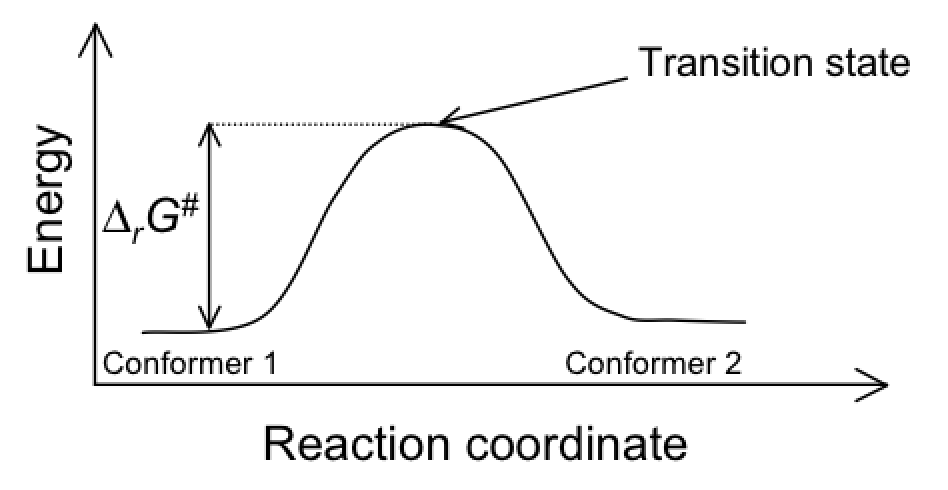
\includegraphics[scale=0.5]{fig8}
\caption{Definition of the Gibbs energy of activation. Note that the effects of the zero-point energies etc. effects are not shown. The reaction coordinate corresponds to the internal mode of rotation.}
\label{fig8}
\end{center}
\end{figure}

\noindent
This can be rewritten in terms of natural logarithms:

\begin{equation}
\underbrace{\ln\left(\frac{k_1}{T}\right)}_{``y''} = \underbrace{-\left(\frac{\Delta_rH^\#}{R}\right)}_{``k''}\times\underbrace{\left(\frac{1}{T}\right)}_{``x''} + \underbrace{\frac{\Delta_rS^\#}{R} + \ln\left(\frac{k_B}{h}\right)}_{``b''}
\label{eq19}
\end{equation}

\noindent
Plotting $\ln(k_1 / T)$ vs. $T^{-1}$ will yield a straight line with a slope $-(\Delta_rH^\# / R)$ and a constant factor that is directly related to the entropy of activation. Thus the fit yields experimental estimates for these quantities.

How is the activation enthalpy related to the activation energy in Eq. (\ref{eq16})? The formal definition of the activation energy $E_A$ gives the following result:

\begin{equation}
E_A = RT^2\ln\left(\frac{\partial\ln(k_1)}{\partial T}\right) = \Delta_rH^\# + RT
\label{eq20}
\end{equation}

\section{Experimental}

\noindent
\underline{Task overview:} In this experiment time-domain (i.e., pulsed) NMR spectroscopy will be used to record NMR spectra of DMF at various temperatures.
Sample preparation: A 10 mL solution of 0.02 M DMF is prepared using perdeuterated nitrobenzene as the solvent. A small quantity is placed in an NMR tube, which is then placed in a ceramic spinner to calibrate the exposed length. Once properly prepared, it is placed in the NMR instrument.\\

\noindent
\underline{Instrument:} The NMR spectra are taken with the Bruker DRX 400 instrument operating at 400 MHz. This is a variable temperature, high-resolution instrument capable of measuring spectra of many nuclei, including hydrogen. Blowing cold or warm gaseous nitrogen on the sample can be used to control the temperature. When the sample spectrum is desired, one must first maximize the absorption signal by ensuring that the magnetic field is uniform (``shimming''). To do this one must adjust the shims of the magnet and then lock the signal. Lock on the deuterium signal from deuterated nitrobenzene. After this the signal can be maximized through various amplification procedures.\\

\noindent
\underline{Measurements:} The NMR spectra should be recorded at 298, 313, 343, 373, 393 and 413 K. After the bands are recorded be sure to note the chemical shift and the FWHM values for the peaks. Also print out paper copies of the spectra.

\section{Data analysis}

First analyze one of the NMR spectra in the slow exchange regime (use the chemical shifts given in Table \ref{table1}) and note the relative intensities of the peaks. Based on this, identify the resonances for the methyl protons. These are the two resonances that will experience temperature dependent behavior. Note that the spin-spin couplings are not visible in the spectra.

Categorize the NMR spectra into the three cases: 1) slow exchange, 2) intermediate exchange, and 3) fast exchange. Be sure to remove the residual linewidth from your data. At 300 K you may assume that exchange does not occur and you obtain a natural linewidth for your sample. This residual linewidth, which is not related to the exchange process, should be subtracted from each $\Delta\nu_{1/2}$ value at every temperature:

\begin{equation}
\Delta\nu_{1/2}(T) = \Delta\nu_{1/2,obs}(T) - \Delta\nu_{1,2,obs}(\textnormal{300 K})
\label{eq21}
\end{equation}

\noindent
where subscript obs refers to values obtained from the NMR spectra and $\Delta\nu_{1/2}$ is the value to be used with Eqs. (\ref{eq12}) and (\ref{eq14}). In case 1), use Eq. (\ref{eq12}) to obtain the conformer lifetimes ($\Delta t$), in case 2) attempt to locate the point of coalescence and use Eq. (\ref{eq13}) to obtain $\Delta t$, and in 3) use the Eq. (\ref{eq14}). Prepare a table with the sample temperature (K) and the inverse of the conformer lifetime ($1 / \Delta t$) (s$^{-1}$). Transform (``Table$\rightarrow$Set Column Values...'') the column 1 to correspond to 1/col("1") (i.e., $1/T$) and for column 2 to ln(col("1")*col("2")) (i.e., $\ln(k_1/T)$). These columns now correspond to ``x'' and ``y'' in Eq. (\ref{eq19}).

Fit the tabulated data to Eq. (\ref{eq19}) and obtain experimental estimates for $\Delta_rH^\#$, $\Delta_rS^\#$ and $\Delta_rG^\#$. Use Eq. (\ref{eq20}) to obtain the activation energy $E_A$. Use the qtiplot program to fit your data. Enter your data into the empty table in qtiplot and choose ``Analyze $\rightarrow$ Fit Linear'' to perform the linear least squares fit. The results (i.e., the slope and the intercept) along with their error estimates are shown in the Results.log window (you may have to scroll the window up to see the results). Be sure to convert these values to the actual $\Delta_rH^\#$ and $\Delta_rS^\#$ values by using Eq. (\ref{eq19}). Use the least squares estimates to provide statistical errors for $\Delta_rH^\#$ and $\Delta_rS^\#$.

\section{Written laboratory report}

Follow the general instructions for written laboratory reports. In addition, include the requested data in the following section:\\

\noindent
\underline{Results.} This section must include the values and error estimates for the values of $\Delta_rG^\#$, $\Delta_rH^\#$, $\Delta_rS^\#$ and $E_A$. Present also literature values for these quantities \cite{JONAS}. Discuss the possible sources of error.

\section{References}

\vspace{-1cm}

\bibliography{../references}

\end{document}
